\chapter{The LHC and The CMS Experiment}

\section{The LHC}
The Large Hadron Collider(LHC) is the largest and most powerful superconducting hadron accelerator and collider. The LHC was installed in an existing 26.7 km tunnel that was constructed for LEP machine between 1984 and 1989. 
\subsection{LHC: Performance and Main machine layout}

\begin{figure}[htbp]
 \begin{center}
  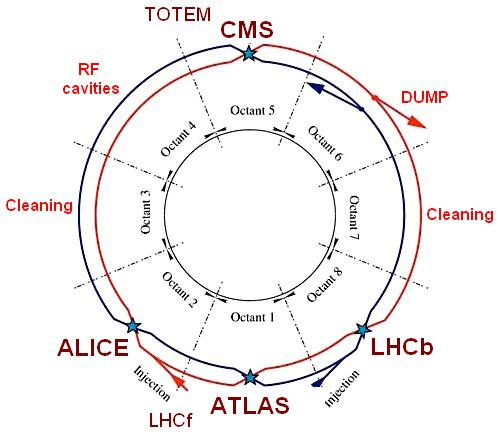
\includegraphics[width=0.8\textwidth]{figures/c3/c3_lhc_latticelayout.jpg}
 \end{center}
 \caption{abcf}
 \label{fig:c3lhclayout}
\end{figure}

Performance, eq, lumi, xsection. Lumi equation from lhc parameter.
Main machine layout: 2 beam with 2 rings, 8 long straight sections and 8 arcs.

\begin{equation}
 L = \frac{N^{2}_{b}n_{b}f_{rev}\gamma_{r}}{4\pi \varepsilon_{n}\beta *}F \;
 \label{eq:c3lhclumi}
\end{equation}

\begin{equation}
 F = (1+\frac{\theta_{c}\sigma_{c}}{2\sigma *})^{-1/2} \;
 \label{eq:c3lhcgeof}
\end{equation}

\subsection{LHC: From operation point of view}
LHC accelerator mode and beam mode. 

\section{The CMS Experiment}

\subsection{CMS Detector System}
\subsubsection{Inner Trackers}
\paragraph{Silicon Pixels}
\paragraph{Silicon Strips}

\subsubsection{Calorimeters}
\paragraph{Electromagnetic Calorimeter}
\paragraph{Hadron Calorimeter}

\subsubsection{Muon Detectors}
\paragraph{Muon Drift Tubes}
\paragraph{Cathode Strip Chambers}
\paragraph{Resistive Plate Chambers}

\subsection{Event Reconstrunction}
\subsubsection{Particle Flow}
\subsubsection{Tracks}
\subsubsection{Electrons}
\subsubsection{Muons}
\subsubsection{Jets and Missing Transverse Energy}
